\section{先行研究}

\subsection{クラスタリング}
クラスタリングとはデータを教師なし学習により任意の数のクラスタに分ける手法である.
クラスタとは,データのグループである.
多くのクラスタリング手法において,ユークリッド距離やマハラノビス距離などの距離尺度を用い,データからクラスタを抽出する.
クラスタリングはデータ解析,データマイニング,画像処理,パターン認識など様々な分野で用いられる.

\subsection{K-means}
%k-meansのkは$k$
様々なクラスタリング手法の中で最も有名な手法がk-meansである.
K-means$^{1)}$は,多次元空間上のデータについて,ユークリッド距離を用い各データ点が属するクラスタを決定する手法である.
% K-meansは,以下の2つの手順を繰り返すことでクラスタリングを行う.
% \begin{enumerate}
%   \item 各データ点とデータ点の距離を求め,各データ点を最も近いセントロイドのクラスタに割り当てる.
%   \item クラスタに所属するデータの平均を新たなセントロイドとする.
% \end{enumerate}
% セントロイドが移動しなくなったらクラスタリングを終了する.

$D$次元空間上の確率変数$\vector{x}$の$N$個のデータ点で構成されるデータ
$\{\vector{x}_1, \vector{x}_2, \cdots, \vector{x}_N\}$があるとする.
このデータを$K$個のクラスタに分割することを考える.
ここで,セントロイド$\vector{\mu}_k$を導入する.セントロイド$\vector{\mu}_k$とはクラスタの重心を表す.
K-meansはクラスタに所属するデータ点とそのクラスタのセントロイド間のユークリッド距離の総和を最小にすることで,クラスタリングを行う.

ここで,各データ点$\vector{x}_n$に対し,対応する2値指示変数$r_{nk} \in \{0, 1\}\ (k = 1, \cdots, K)$を定める.
これは,そのデータ点$\vector{x}_n$がクラスタ$k$に割り当てられるかを表す変数である.
すなわち,データ点$\vector{x}_n$がクラスタ$k$に割り当てられる場合は$r_{nk}=1$とし,
そうでない場合は$r_{nk}=0$とする.これは,1-of-K符号化法として知られている.

次に,$k$-meansにおける目的関数$J$を定義する.
\begin{align}
  \label{eq:J-func}
  J = \sum_{n=1}^{N} \sum_{k=1}^{K} r_{nk} \| {\displaystyle \vector{x}_n - \vector{\mu}_k} \|^2
\end{align}
これは,各データ点からそれらが割り当てられたクラスタのセントロイド$\vector{\mu}_k$までのユークリッド距離の2乗の総和を表している.%ユークリッド距離が嫌ならL2ノルム
K-meansによるクラスタリングは,$J$を最小にする$\{r_{nk}\}$と$\{\vector{\mu}_k\}$の値を求めることに換言できる.

まず$r_{nk}$の決定を考える.
\eqref{eq:J-func}における$J$は$r_{nk}$についての線形関数なので,最適化は代数的に解くことができる.
異なる$n$を含む項は互いに独立である.よって,各$n$について別々に$r_{nk}=1$としたときに,
$||\vector{x}_n - \vector{\mu}_k||^2$が最小になるような$k$の値に対して$r_{nk}$を選んで1とおけばよい(\eqref{eq:rnk}).
\begin{align}
  \label{eq:rnk}
  r_{nk} = \left\{
    \begin{array}{ll}
      1 & k = \arg\min_j \|\vector{x}_n - \vector{\mu}_j\|  \text{のとき}\\
      0 & \text{それ以外}
    \end{array}
  \right.
\end{align}
つまり,単純に$n$番目のデータ点がそれに最も近いセントロイドを持つクラスタに割り当てるのである.

次に,$r_{nk}$を固定したもとで$\vector{\mu}_k$の最適化を考える.
対象関数$J$は$\vector{\mu}_k$の二次関数であり,次のように$\vector{\mu}_k$に関する偏微分を0とおく事で最小化できる
(\eqref{eq:mu-dif}).
\begin{align}
  \label{eq:mu-dif}
  2\sum_{n=1}^n r_{nk}(\vector{x}_n - \vector{\mu}_k) = 0
\end{align}
これを$\vector{\mu}_k$についてとくと,\eqref{eq:mu}を得る.
\begin{align}
  \label{eq:mu}
  \vector{\mu}_k = \frac{\sum_n r_{nk}\vector{x}_n}{\sum_n r_{nk}}
\end{align}
この式の分母は$k$番目のクラスタに割り当てられたデータの数に等しい.
それゆえ$\vector{\mu}_k$は$k$番目のクラスタに割り当てられた全てのデータ点$\vector{x}_n$の
平均値と単純に解釈することができる.

\begin{figure}[htbp]
  \begin{minipage}{0.33\hsize}
    \begin{center}
      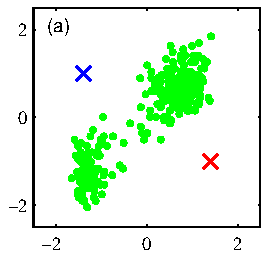
\includegraphics[width=40mm]{img/kmeans/Figure91a.pdf}
    \end{center}
  \end{minipage}
  \begin{minipage}{0.33\hsize}
    \begin{center}
      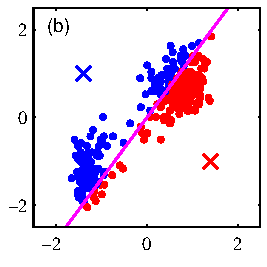
\includegraphics[width=40mm]{img/kmeans/Figure91b.pdf}
    \end{center}
  \end{minipage}
  \begin{minipage}{0.33\hsize}
    \begin{center}
      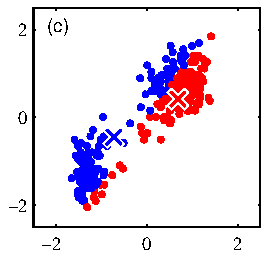
\includegraphics[width=40mm]{img/kmeans/Figure91c.pdf}
    \end{center}
  \end{minipage}\\
  \begin{minipage}{0.33\hsize}
    \begin{center}
      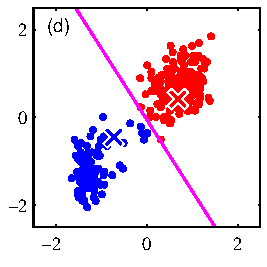
\includegraphics[width=40mm]{img/kmeans/Figure91d.pdf}
    \end{center}
  \end{minipage}
  \begin{minipage}{0.33\hsize}
    \begin{center}
      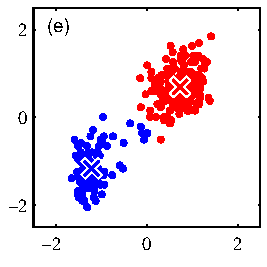
\includegraphics[width=40mm]{img/kmeans/Figure91e.pdf}
    \end{center}
  \end{minipage}
  \begin{minipage}{0.33\hsize}
    \begin{center}
      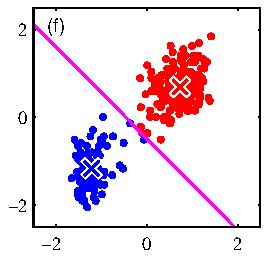
\includegraphics[width=40mm]{img/kmeans/Figure91f.pdf}
    \end{center}
  \end{minipage}\\
  \begin{minipage}{0.33\hsize}
    \begin{center}
      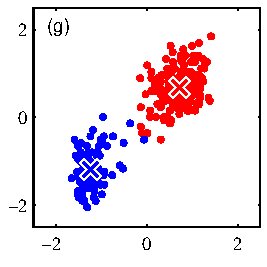
\includegraphics[width=40mm]{img/kmeans/Figure91g.pdf}
    \end{center}
  \end{minipage}
  \begin{minipage}{0.33\hsize}
    \begin{center}
      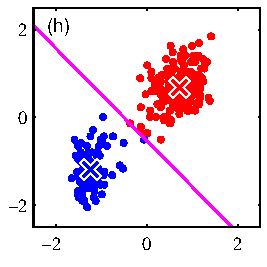
\includegraphics[width=40mm]{img/kmeans/Figure91h.pdf}
    \end{center}
  \end{minipage}
  \begin{minipage}{0.33\hsize}
    \begin{center}
      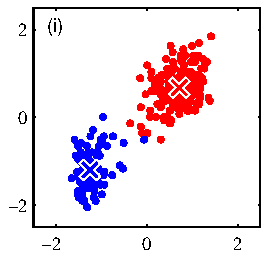
\includegraphics[width=40mm]{img/kmeans/Figure91i.pdf}
    \end{center}
  \end{minipage}
  \caption{K-meansの動作}
  \label{fig:k-means}
\end{figure}

\figurenum{fig:k-means}にK-meansによるクラスタリングの具体例を示す.
K-meansでは,$r_{nk}$と$\vector{\mu}_k$をそれぞれ最適化する2つのステップを
交互に繰り返す手続きでクラスタリングを実現する.

最初に,$\vector{\mu}_k$の初期値を選ぶ(a).
次に,最初のフェーズで$\vector{\mu}_k$を固定しつつ,$r_{nk}$について$J$を最小化する(b).
第二フェーズでは,$r_{nk}$を固定しつつ,$\vector{\mu}_k$について$J$を最小化する(c).
そして,このような二段階最適化を収束するように繰り返す.

データ点のクラスタへの再割り当てと,クラスタ平均の再計算という2つのフェーズは,
再割当てが起こらなくなるまで(もしくはあらかじめ定めた最大繰り返し数を超えるまで)繰り返される.
各フェーズは,対象関数$J$の値を減少させるので,このアルゴリズムの収束は保証されている.
しかしながら,大域的最小点ではなく極小点に収束する可能性はある.

なお,K-meansによるクラスタリングは,事前にクラスタ数を指定することによりクラスタリングを行うため
クラスタ数が未知の場合,K-meansを用いることはできない.

\subsection{Kullback-Leibler情報量}
偶然を伴う現象は,ある確率分布に従う確率変数の実現値であると考えることができる.
この確率分布を近似するモデル(以後「モデル」)は,データを生成する真の確率分布に
どの程度近いかによって評価することができる.
また,データにモデルを当てはめることは,データから真の確率分布を推定しているものと
みなすことができる.このようにモデルと真の分布が共に確率分布であると見なし,
モデルの評価や推定を行う.

真の分布とモデルの近さを測る客観的な規準としてKullback-Leibler情報量(以後「K-L情報量」)がある.
連続型の確率分布のとき,$g(x)$を真の確率密度関数,$f(x)$をモデルが定める確率密度関数とすると,
モデルに関する真の分布のK-L情報量は$\log\{g(X)/f(X)\}$の期待値を取り\eqref{eq:k-l-div}で表される.
\begin{align}
  \label{eq:k-l-div}
  I(g \mid f) &= E_X\left(\log \left\{\frac{g(X)}{f(X)}\right\}\right)\\\nonumber
              &= \int^{\infty}_{-\infty}\log\left\{\frac{g(x)}{f(x)}\right\}g(x)dx
\end{align}
ただし,$\log$は自然対数で,注記がない限り一貫してこの意味で用いる.

このように,真の分布がわかっている場合にはK-L情報量によってモデルの良し悪しを比較できた.
しかし,通常は真の分布が未知で,真の分布から得られたデータだけが与えられていることがい.
したがって,データからK-L情報量を推定する必要がある.
\eqref{eq:k-l-div}を展開すると
\begin{align*}
  I(g \mid f) &= \int^{\infty}_{-\infty}\left\{\log\frac{g(x)}{f(x)}\right\}g(x)dx\\\nonumber
              &= -\int^{\infty}_{-\infty}\{\log f(x)\}g(x)dx - 
                 \left(-\int^{\infty}_{-\infty}\{\log g(x)\}g(x)dx\right)
\end{align*}
となるが,右辺の第2項は定数であり,右辺第1項が大きいほどK-L情報量$I(g \mid f)$は
小さくなることがわかる.
すなわち,K-L情報量の大小比較のためには,本質的には$\int^{\infty}_{-\infty}\{\log f(x)\}g(x)dx$だけを推定すれば良いことがわかる.
右辺第1項の$\int^{\infty}_{-\infty}\{\log f(x)\}g(x)dx$は,確率密度関数$\log f(x)$の期待値$E( \log f(x))$であり,平均対数尤度と呼ばれている.
ここで,
\begin{align*}
  \sum_{i=1}^{n}\log f(x_i)
\end{align*}
を対数尤度と呼ぶことにすると,$n$個の独立な観測値$\{x_1, x_2, \cdots, x_i\}$が得られると,
この平均対数尤度は,対数尤度の$n$分の1
\begin{align*}
  \frac{1}{n}\sum_{i=1}^{n}\log f(x_i)
\end{align*}
で近似される.
したがって,符号に注意すると,対数尤度が大きいほど,そのモデルは真の分布に近いと考えられる.
このようにして,対数尤度をK-L情報量の推定値と考えることにすると異なったタイプのモデルの
良し悪しも比較できるのである.

ところで,確率変数$(X_1, X_2, \cdots, X_n)$の同時密度関数が$f(x_1, x_2, \cdots, x_n \mid \theta)$で
与えられているものとする.
$\theta$は確率密度関数を規定するパラメータである.この時,観測値$(x_1, x_2, \cdots, x_n)$は
与えられたものとして固定し,$f$を$\theta$の関数と考える時,この関数を\textbf{尤度}と呼び,
$L(\theta)$で表す.すなわち,
\begin{align*}
  L(\theta) = f(x_1, x_2, \cdots, x_n \mid \theta)
\end{align*}
である.特に,確率変数が独立な場合には$(X_1, X_2, \cdots, X_n)$の確率密度関数は,
各$X_i (i = 1, \cdots, n)$の確率密度関数の積に等しいことから,
\begin{align*}
  L(\theta) = f(x_1 \mid \theta)f(x_2 \mid \theta) \cdots f(x_n \mid \theta)
\end{align*}
となる.この両辺の対数をとると,すでに求められた対数尤度関数
\begin{align*}
  l(\theta) = \sum_{i=1}^{n}\log f(x_i \mid \theta)
\end{align*}
が導かれる.

ここでは,平均対数尤度の推定量から対数尤度を直接導入した.
しかし,モデルが確率分布の形で与えられている場合には,まず観測値の同時分布から
尤度を定義し,その対数として対数尤度を求めるほうが都合が良い.
$(X_1, X_2, \cdots, X_n)$が独立でない場合にも,尤度の対数として対数尤度
\begin{align*}
  l(\theta) = \log f(x_1, \cdots, x_n \mid \theta)
\end{align*}
が定義できる.

\subsection{最尤法}
ここまで,データに基づいてK-L情報量の大小を比較するためには対数尤度を比較すれば良いことを示した.
あらかじめ与えられたいくつかのモデルがある場合には,対数尤度が最大となるモデルを選択することによって,
近似的には真の分布にいちばん近いモデルが得られることになる.
したがって,モデルがいくつかの調整できるパラメータを保つ場合には,対数尤度を最大とするように
パラメータの値を選ぶことによって良いモデルが得られることがわかる.
この推定を最大尤度法,略して\textbf{最尤法}と呼ばれている.
また,最尤法で導かれた推定量は\textbf{最尤推定量}と呼ばれ,この最尤推定量によって定められるモデルが
最尤モデルである.
最尤モデルの対数尤度を\textbf{最大対数尤度}という.
